\section{External Interface Requirements}

\subsection{User Interfaces}
Vai Brio tocca a te


\subsection{Hardware Interfaces}
The system does not need any specific hardware, each user will need a browser with an Internet connection in order to communicate with the servers of the platform.

\subsection{Software Interfaces}
To do

\subsection{Comunication Interfaces}
\begin{enumerate}
    \item \textbf{eduGAIN Radius} - in order to allow a native single sign-on for all European universities.
    \item \textbf{OAuth2} - is a very commonly used standard in the enterprise environment, to consent the adoption of Single Sign On (SSO) with external platform.
    \item \textbf{HyperText Transfer Protocol over Secure Socket Layer (HTTPS)} - used for all communications between client  and server.
    \item \textbf{Simple Mail Transfer Protocol (SMTP)} - , a standard protocol for email transmission, which is used by this platform to send notifications through email.
\end{enumerate}

\section{Functional Requirements}
\begin{enumerate}[label=\textbf{R\arabic*}:,ref=R\arabic*,leftmargin=1.3cm]
    \labelleditem{The system shall allow students to log in with SSO.}
    \labelleditem{The system shall allow company employee to log in with SSO.}
    \labelleditem{The studens shall allow the student to provide information about their CVs.}
        \begin{enumerate}[label=\textbf{R\arabic{enumi}.\arabic*}:,ref=R\arabic{enumi}.\arabic*, leftmargin=*]
            \labelledsubitem{The system shall allow the students to specify their personal information, like name, contact and personal ambition.}
            \labelledsubitem{The system shall allow the students to specify their education experience, like the academic background.}
            \labelledsubitem{The system shall allow the students to specify their passed work experience, specifying job title, company name, duration and technologies used.}
            \labelledsubitem{The system shall allow the students to specify their technical and soft skills.}
            \labelledsubitem{The system shall allow the students to specify their project and research, including the title, duration and description}
            \labelledsubitem{The system shall allow the students to specify their extracurricular activities, including the name, organization and achievements.}
            \labelledsubitem{The system shall allow the students to specify their knowledge of languages, including the level and eventual certifications.}
            \labelledsubitem{The system shall allow the students to specify their availability.}
            \labelledsubitem{The system shall allow the students to specify their additional information.}
        \end{enumerate}
    \labelleditem{The system shall allow the students to join an internship.}
        \begin{enumerate}[label=\textbf{R\arabic{enumi}.\arabic*}:,ref=R\arabic{enumi}.\arabic*, leftmargin=*]
            \labelledsubitem{The system shall help the user to create a customized CV for each company.}
            \labelledsubitem{The system shall allow the students to be notified when a new probably interesting internship becomes available.}
        \end{enumerate}
    \labelleditem{The system shall allow the company employee to create an internship.}
        \begin{enumerate}[label=\textbf{R\arabic{enumi}.\arabic*}:,ref=R\arabic{enumi}.\arabic*, leftmargin=*]
            \labelledsubitem{The system shall allow the company employee to specify the title of the internship.}
            \labelledsubitem{The system shall allow the company employee to specify the description of the internship.}
            \labelledsubitem{The system shall allow the company employee to specify the requirement of the internship.}
            \labelledsubitem{The system shall allow the company employee to specify the duration of the internship.}
            \labelledsubitem{The system shall allow the company employee to specify the availability of the internship.}
            \labelledsubitem{The system shall allow the company employee to specify other information about the internship.}
            \labelledsubitem{The system shall allow the company employee to be notified when a new probably interesting student becomes available.}
        \end{enumerate}
    \labelleditem{The system shall allow the company to open a claim to the university.}
    \labelleditem{The system shall allow the students to open a claim to the university.}
    \labelleditem{}{The system shall allow students to chat with his company.}
    \labelleditem{The system shall allow employee to chat with his students.}
\end{enumerate}

\subsection{Use case diagrams}
\subsection{Use cases}

    \textbf{UC1}
    \begin{table}[H]
    \centering
    \begin{tabular}{|l|p{11.9cm}|}
        \hline
        \textbf{Name}            & Student's first platform access                     \\\hline
        \textbf{Actor}           & Student         \\\hline
        \textbf{Entry condition} &
        \begin{itemize}
              \item Student has never accessed the platform
        \end{itemize}                                        \\\hline
        \textbf{Event flow}      &
        \begin{enumerate}[label=\arabic*.]
              \item The student, who has got an internet connection, insert the URL in the browser.
              \item The student clicks on the login button.
              \item The student inserts his email and will be redirected to the university SSO.
              \item The students selects his favorite academic interests.
        \end{enumerate}            \\\hline
        \textbf{Exit condition}  & The students is redirected to the homepage\\\hline
        \textbf{Exception}       &  Student's credentials are not valid. In this case a pop up will be shown.   \\\hline
    \end{tabular}
    \caption{Student's first platform access}
    \label{table:Student's first platform access}
    \end{table}

    \begin{figure}[H]
        \centering
        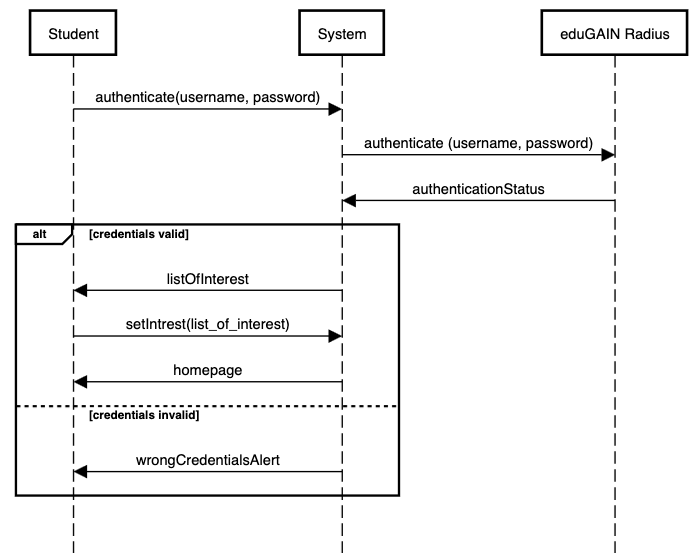
\includegraphics[width=0.8\textwidth]{Assets/SequenceDiagrams/1-login.png}
        \caption{Student's first platform access.}
        \label{fig:Student's first platform access}
    \end{figure}

    \textbf{UC2}
    \begin{table}[H]
    \centering
    \begin{tabular}{|l|p{11.9cm}|}
        \hline
        \textbf{Name}            & Student provides his CV’s information to the platform \\\hline
        \textbf{Actor}           & Student         \\\hline
        \textbf{Entry condition} &
        \begin{itemize}
              \item Student is already logged in
              \item Student has never provided his information in "My CV" section
        \end{itemize}                                        \\\hline
        \textbf{Event flow}      &
        \begin{enumerate}[label=\arabic*.]
            \item The student press on the contact button.
            \item The student, altered by a pop-up, follows the redirect to the "My CV" page.
            \item The student fills out the form.
            \item The student click on the save button.
        \end{enumerate}            \\\hline
        \textbf{Exit condition}  & The system will show a message confirming the success of the operation.\\\hline
        
        \textbf{Exception}       &  Student misses to compile some fields. In this case, an alert pop-up is shown.  \\\hline
    \end{tabular}
    \caption{Student provides his CV’s information to the platform.}
    \label{table:Student provides his CV’s information to the platform}
    \end{table}

    \begin{figure}[H]
        \centering
        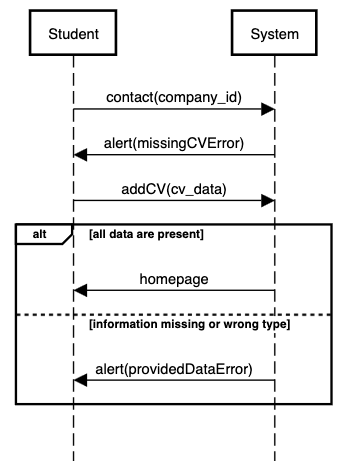
\includegraphics[width=0.8\textwidth]{RASD/Assets/SequenceDiagrams/2-student-provide-his-cv.png}
        \caption{Student provides his CV’s information to the platform.}
        \label{fig:Student provides his CV’s information to the platform}
    \end{figure}


    \textbf{UC3}
    \begin{table}[H]
    \centering
    \begin{tabular}{|l|p{11.9cm}|}
        \hline
        \textbf{Name}            & Student search and contact the company \\\hline
        \textbf{Actor}           & Student, Company Employee         \\\hline
        \textbf{Entry condition} &
        \begin{itemize}
              \item Student is already logged in
              \item Student has already compiled his Curriculum Vitae
        \end{itemize}                                        \\\hline
        \textbf{Event flow}      &
        \begin{enumerate}[label=\arabic*.]
              \item The student opens the homepage.
              \item The student click on contact button next to the interested company.
              \item The platform generate a customized CV.
              \item The student reads the proposal customized and send it.
              \item The company receive the customized CV.
        \end{enumerate}            \\\hline
        \textbf{Exit condition}  & The company employee approve student's CV.\\\hline
        \textbf{Exception}       &  
        \begin{itemize}
              \item The student does not appreciate the customized CV proposed by the platform. In this case, the student manually modify it.
              \item The company employee does not approve the student's CV. In this case, the employee can reject the proposal.  
        \end{itemize} 
        \\\hline
    \end{tabular}
    \caption{Student search and contact the company}
    \label{table:Student search and contact the company}
    \end{table}

    \begin{figure}[H]
        \centering
        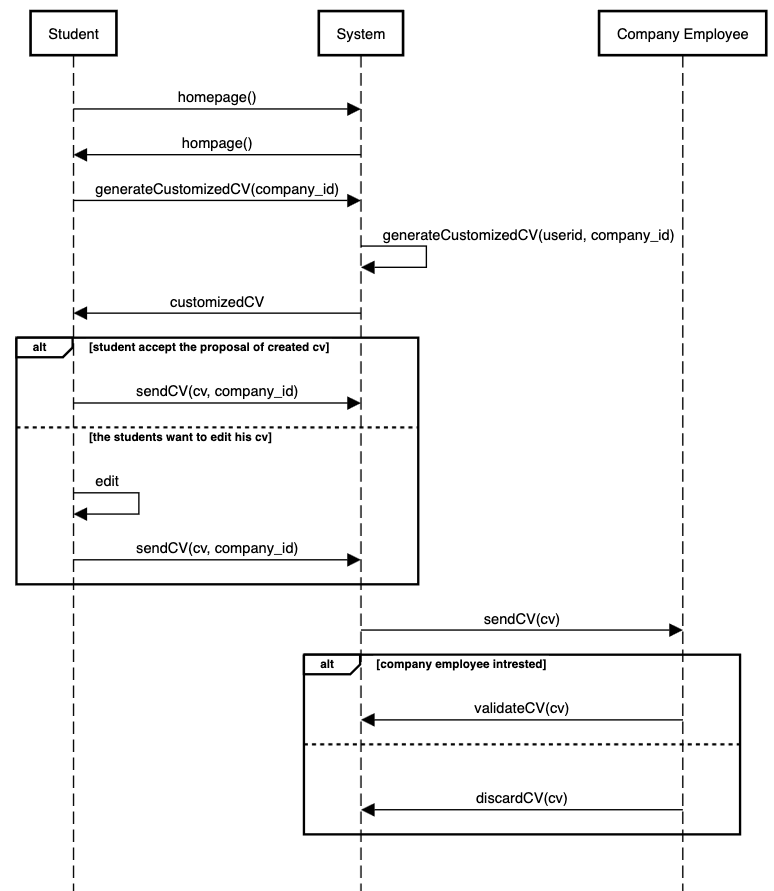
\includegraphics[width=0.8\textwidth]{RASD/Assets/SequenceDiagrams/3-student-contact-company.png}
        \caption{Student search and contact the company.}
        \label{fig:Student search and contact the company}
    \end{figure}

    
    \textbf{UC4}
    \begin{table}[H]
    \centering
    \begin{tabular}{|l|p{11.9cm}|}
        \hline
        \textbf{Name}            & A company publishes an advertisement about the internships they are
offering \\\hline
        \textbf{Actor}           & Company Employee, Student possibly interested on that opportunity.        \\\hline
        \textbf{Entry condition} &
        \begin{itemize}
              \item Company was already approved on the platform
        \end{itemize}                                        \\\hline
        \textbf{Event flow}      &
        \begin{enumerate}[label=\arabic*.]
              \item The company employee logs in using his company's credentials.
              \item The company employee opens the "Create Job Opportunity" page.
              \item The company employee insert into the platform all the information requested.
              \item A successful message is show, and, after a couple of second, the company employee is redirected to the hompage.
        \end{enumerate}            \\\hline
        \textbf{Exit condition}  & Interested students receive a notification \\\hline
        \textbf{Exception}       &  Company employee has not full field the form. In this case, an alert message is shown.   \\\hline
    \end{tabular}
    \caption{Student search and contact the company}
    \label{table:Student search and contact the company}
    \end{table}

    \begin{figure}[H]
        \centering
        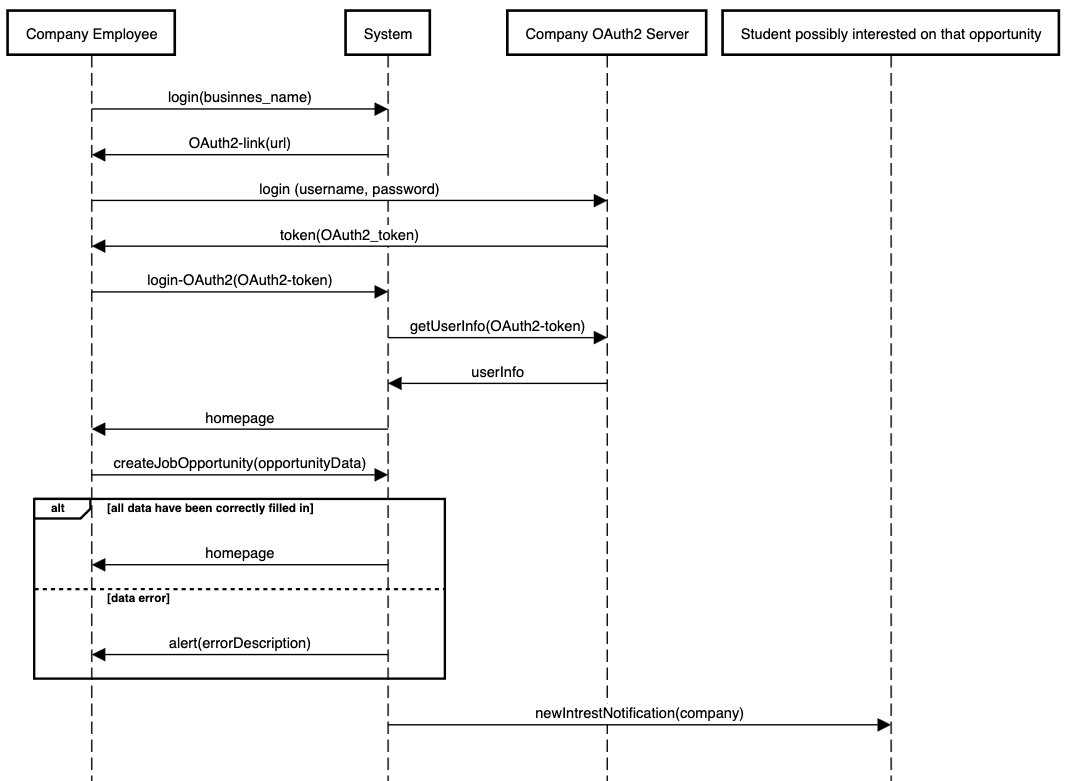
\includegraphics[width=0.8\textwidth]{RASD/Assets/SequenceDiagrams/4-company-publish-and-adv.png}
        \caption{Student search and contact the company.}
        \label{fig:Student search and contact the company}
    \end{figure}


    \textbf{UC5}
    \begin{table}[H]
    \centering
    \begin{tabular}{|l|p{11.9cm}|}
        \hline
        \textbf{Name}            & Student search and contact the company \\\hline
        \textbf{Actor}           & Student, Company Employee         \\\hline
        \textbf{Entry condition} &
        \begin{itemize}
              \item Student is already logged in
              \item Student has already compiled his Curriculum Vitae
              \item A Company has published an internship may interest the student.
        \end{itemize}                                        \\\hline
        \textbf{Event flow}      &
        \begin{enumerate}[label=\arabic*.]
              \item The student receive an email.
              \item The student click on the link contained in the email.
              \item The student is interested on that specific internship, so he press on "Contact" button.
              \item The student appreciates the custom generated CV.
        \end{enumerate}            \\\hline
        \textbf{Exit condition}  & Student clicks in "Send" button.\\\hline
        \textbf{Exception}       &  
        \begin{itemize}
            \item The student is not interested on the proposed internship. In this case, the student just ignore the notification.
            \item The student does not appreciate the customized CV proposed by the platform. In this case, the student manually modify it.
        \end{itemize} 
        \\\hline
    \end{tabular}
    \caption{Student search and contact the company}
    \label{table:Student search and contact the company}
    \end{table}
oi
    \begin{figure}[H]
        \centering
        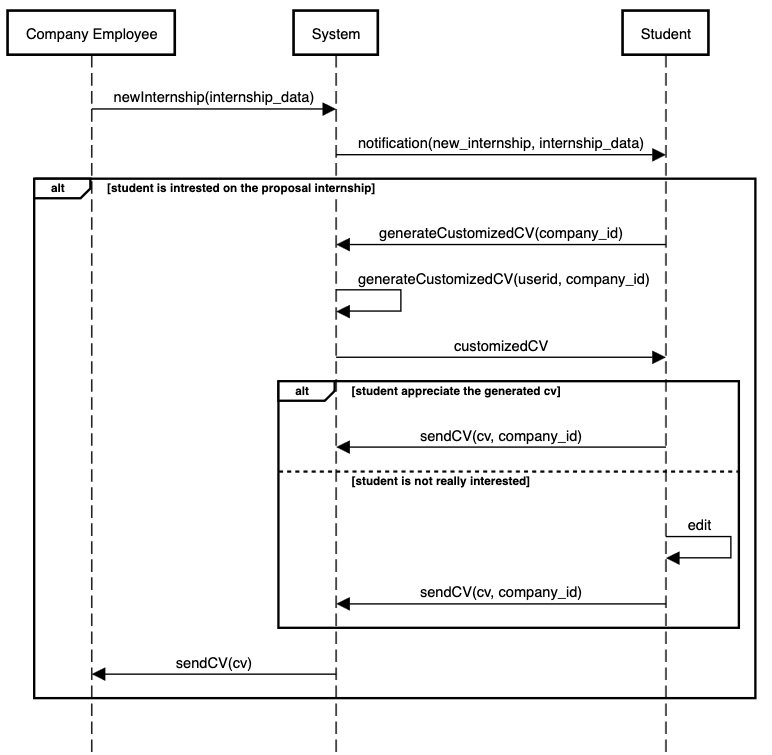
\includegraphics[width=0.8\textwidth]{RASD/Assets/SequenceDiagrams/5-student-receives-a-notification.png}
        \caption{Student receive a notification about the availability of an internship that might interest him.}
        \label{fig:Student receive a notification about the availability of an internship that might interest him}
    \end{figure}


    \textbf{UC6}
    
    \begin{table}[H]
        \centering
        \begin{tabular}{|l|p{11.9cm}|}
        \hline
        \textbf{Name}            & A company receive a notification about the availability of a student CV corresponding to their needs \\\hline
        \textbf{Actor}           & Student, Company Employee       \\\hline
        \textbf{Entry condition} &
        \begin{itemize}
              \item Students has just completed his "My CV" section
        \end{itemize}                                        \\\hline
        \textbf{Event flow}      &
        \begin{enumerate}[label=\arabic*.]
              \item The system will start a matchmaking process between the student and opened internship positions.
              \item The system sends a notification to all of the Company Employees who may be interested in the new student.
              \item The company employee, who receive the notification, click on the "View Profile" button to obtain more detailed information about his CV.
              \item The company employee click on send message, near the student name, to contact it.
              
        \end{enumerate}            \\\hline
        \textbf{Exit condition}  & The company employee send a message to the student  \\\hline
        \textbf{Exception}       &  The company employee does not really feel interested in the student's proposal. In this case, he just ignored the mail.   \\\hline
        \end{tabular}
        \caption{A company receive a notification about the availability of a student CV corresponding to their needs.}
        \label{table:A company receive a notification about the availability of a student CV corresponding to their needs}
    \end{table}

    \begin{figure}[H]
        \centering
        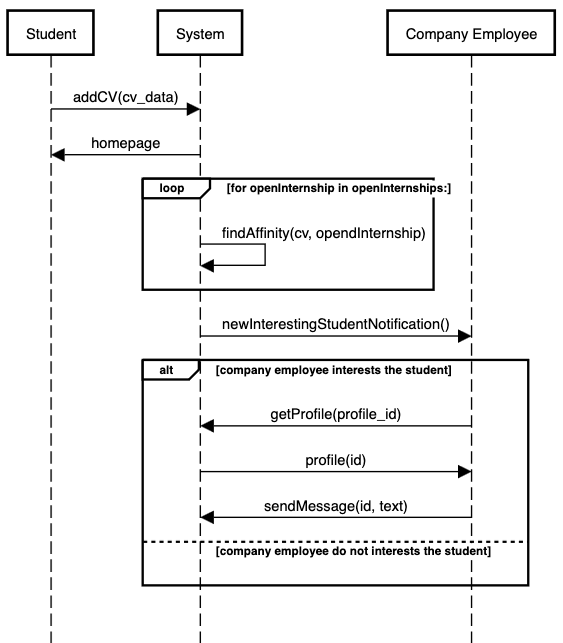
\includegraphics[width=0.8\textwidth]{RASD/Assets/SequenceDiagrams/6-matchmaking-new-student.png}
        \caption{A company receive a notification about the availability of a student CV corresponding to their needs.}
        \label{fig:A company receive a notification about the availability of a student CV corresponding to their needs}
    \end{figure}


    \textbf{UC7}
    
    \begin{table}[H]
        \centering
        \begin{tabular}{|l|p{11.9cm}|}
        \hline
        \textbf{Name}            & Student gives final feedback about the internship \\\hline
        \textbf{Actor}           & Student     \\\hline
        \textbf{Entry condition} &
        \begin{itemize}
              \item Student has just finished his internship
        \end{itemize}                                        \\\hline
        \textbf{Event flow}      &
        \begin{enumerate}[label=\arabic*.]
              \item The student opens the sidebar and click on "Report" button.
              \item The system recognizes that he has just finished an internship, so shows the "Give us your final feedback" form.
              \item The student fills the form.
              
        \end{enumerate}            \\\hline
        \textbf{Exit condition}  & Click on "Submit" button  \\\hline
        \textbf{Exception}       &  The student do not want to provide his feedback. In this case, no action are required.   \\\hline
        \end{tabular}
        \caption{Student gives final feedback about the internship.}
        \label{table:Student gives final feedback about the internship}
    \end{table}

    \begin{figure}[H]
        \centering
        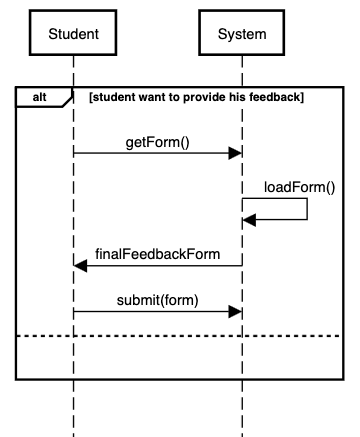
\includegraphics[width=0.8\textwidth]{RASD/Assets/SequenceDiagrams/7-internship-final-form.png}
        \caption{Student gives final feedback about the internship.}
        \label{fig:Student gives final feedback about the internship}
    \end{figure}


    \textbf{UC8}
    
    \begin{table}[H]
        \centering
        \begin{tabular}{|l|p{11.9cm}|}
        \hline
        \textbf{Name}            & University receive the request of ending an internship from a student and contact the company to end it \\\hline
        \textbf{Actor}           & University employee     \\\hline
        \textbf{Entry condition} &
        \begin{itemize}
              \item University employee receives an email 
        \end{itemize}                                        \\\hline
        \textbf{Event flow}      &
        \begin{enumerate}[label=\arabic*.]
              \item The university employee clicks on the "See complain" button in the email, so a new page is opened.
              \item The university employee opens the student's profile by clicking on his name.
              \item The university employee clicks on "Terminate Internship" button.
              
        \end{enumerate}            \\\hline
        \textbf{Exit condition}  & The university employee confirms the pop-up.  \\\hline
        \textbf{Exception}       &    \\\hline
        \end{tabular}
        \caption{University receive the request of ending an internship from a student and contact the company to end it .}
        \label{table:University receive the request of ending an internship from a student and contact the company to end it }
    \end{table}

    \begin{figure}[H]
        \centering
        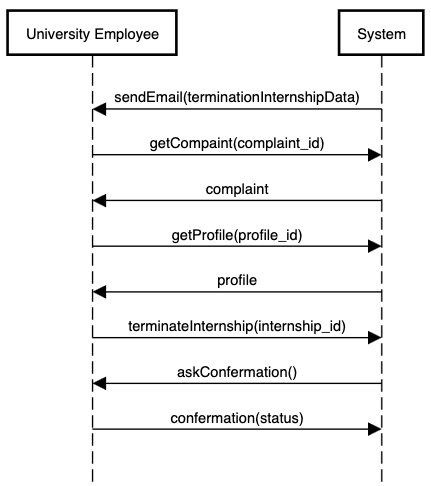
\includegraphics[width=0.8\textwidth]{RASD/Assets/SequenceDiagrams/8-student-end-internship.png}
        \caption{University receive the request of ending an internship from a student and contact the company to end it .}
        \label{fig:University receive the request of ending an internship from a student and contact the company to end it }
    \end{figure}


    \textbf{UC9}
    
    \begin{table}[H]
        \centering
        \begin{tabular}{|l|p{11.9cm}|}
        \hline
        \textbf{Name}            & Student complains with the university on the "Report Area" about his ongoing internship \\\hline
        \textbf{Actor}           & Student    \\\hline
        \textbf{Entry condition} &
        \begin{itemize}
              \item The student is not satisfied with his internship
        \end{itemize}                                        \\\hline
        \textbf{Event flow}      &
        \begin{enumerate}[label=\arabic*.]
              \item The students open the S\&C portal and opens the "Report Area" page.
              \item The student completes the form.
        \end{enumerate}            \\\hline
        \textbf{Exit condition}  & Click on "Submit" button  \\\hline
        \textbf{Exception}       &  The student wants re-try to communicate with his company. In this case, the student will send a message through the chat.   \\\hline
        \end{tabular}
        \caption{Student complains with the university on the "Report Area" about his ongoing internship.}
        \label{table:Student complains with the university on the "Report Area" about his ongoing internship}
    \end{table}

    \begin{figure}[H]
        \centering
        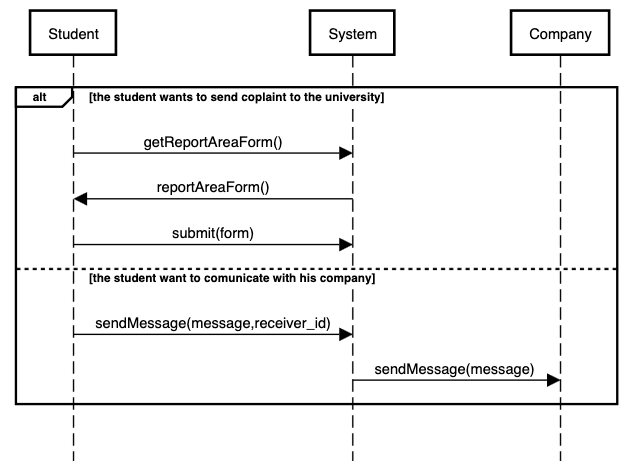
\includegraphics[width=0.8\textwidth]{RASD/Assets/SequenceDiagrams/9-student-sends-a-complaint.png}
        \caption{Student complains with the university on the "Report Area" about his ongoing internship.}
        \label{fig:Student complains with the university on the "Report Area" about his ongoing internship}
    \end{figure}

    \textbf{UC10}
    
    \begin{table}[H]
        \centering
        \begin{tabular}{|l|p{11.9cm}|}
        \hline
        \textbf{Name}            & The company complains about the student taking the internship \\\hline
        \textbf{Actor}           & Company employee, university employee    \\\hline
        \textbf{Entry condition} &
        \begin{itemize}
              \item The company is not satisfied with the student internship
        \end{itemize}                                        \\\hline
        \textbf{Event flow}      &
        \begin{enumerate}[label=\arabic*.]
              \item The company employee open the S\&C portal and opens the "Report Area" page.
              \item The company employee selects the involved student's name.
              \item The company employee clicks on "Report" button in student's page.
              \item The company employee now can fill out the form, describing the problem's detail.
              \item The company employee clicks on "Submit" button
        \end{enumerate}            \\\hline
        \textbf{Exit condition}  & The University receives a notification about the report.\\\hline
        \textbf{Exception}       &  Some form values are missing. In this case, an alert pop-up will be shown.\\\hline
        \end{tabular}
        \caption{The company complains about the student taking the internship.}
        \label{table:The company complains about the student taking the internship}
    \end{table}

    \begin{figure}[H]
        \centering
        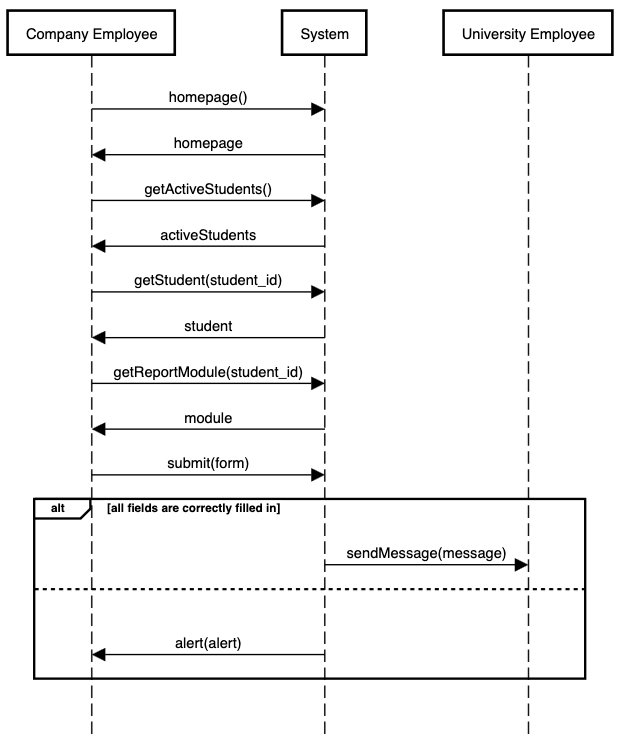
\includegraphics[width=0.8\textwidth]{RASD/Assets/SequenceDiagrams/10-company-sends-a-complaint.png}
        \caption{The company complains about the student taking the internship.}
        \label{fig:The company complains about the student taking the internship}
    \end{figure}